\chapter{Úvod}

\section{Motivácia}
V strojovom učení nastávajú situácie, kedy potrebujeme predikovať výsledok nie len na 
základe aktuálneho vstupu, 
ale aj na základe historického kontextu. Kontextom sú väčšinou stavy modelu z minulých krokov.
Príkladom takejto úlohy môže byť spracovanie tzv. časových radov či generovanie postupností.
Predstavme si úlohu, v ktorej chceme model strojového učenia naučiť predikovať ďalšie písmeno v určitom slove. 
Ako príklad si môžeme zobrať slovo "Bratislava". 
Trénovanie modelu strojového učenia bez využitia kontextu by mohlo prebiehať napríklad takto:
Trénovaciou množinu by tvorili písmená daného slova kde očakávanou hodnotou pre nejaké písmeno by bolo ďalšie písmeno, ktoré za ním v slove nasleduje.
Čiže pre písmeno "B" a poviem, že očakávame "r" a takto pokračujem ďalej cez všetky písmená v slove.

Problém nastane pri druhom písmene "a" v slove Bratislava. Pri prvom výskyte písmena "a" sme modelu tvrdili, že očakávam písmeno "t" a 
pri druhom výskyte písmena "a" tvrdíme, že očakávame "v". 
Tento prípad sa model ktorý nevyužíva žiadny historický kontext, nevie naučiť, pretože nemá žiadnu pamäť (okno do minulosti).

V mojej práci sa budem zaoberať iba jedným modelom strojového učenia, ktorý pracuje s kontextom - rekurentné neurónové siete, konkrétne ich 
pamäťovú hĺbku. Pamäťová hĺbka neurónovej siete vo všeobecnosti vyjadruje to, s akým dlhým kontextom do minulosti dokáže pracovať.

Konkrétne pôjde o nasledujúcim tri typy rekurentných neurónových sietí:
\begin{itemize}
	\item Elmanova sieť
	\item RecSOM
	\item MergeSOM
\end{itemize}

\section{Úvod do neurónových sietí}

\subsection{Perceptrón}
Je základným modelom neurónu, ktorý je používaný v neurónových sietach.

Na vstupe každého perceptrónu je vektor vstupných hodnôt (vzor) $\overline{x}$ pričom hodnoty sú reálne čísla alebo binárne hodnoty, v ktorých môže byť zakódované
napríklad slovo alebo obrázok. Každý perceptrón má vektor synaptických váh $\overline{w}$. 

Výstup perceptrón vyjadruje rovnica:
\begin{equation}
	y = f (\sum_{j=1}^{n+1} w_{i} x_{j}) \quad x_{n+1} = -1
\end{equation}
Funkcia $f$ sa nazýva aj aktivačná funkcia perceptrónu, ktorá môže byť spojitá alebo diskrétna. 
Podľa toho, či je  aktivačná funkcia spojitá a lebo diskrétna, rozlišujeme spojitý alebo diskrétny
perceptrón.

\begin{figure}[H]
	\centering
	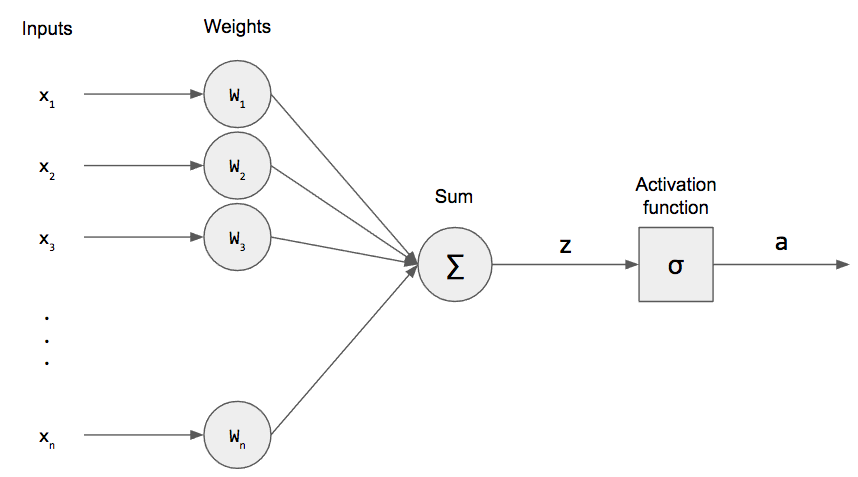
\includegraphics[width=8cm]{assets/perceptron}
	\caption{Percetrón}
\end{figure}

Aktivačná funkcia diskrétneho perceptrónu je jednoduchá bipolárna funkcia, ktorá vráti +1 alebo 1.

\[
f(net) = sign(net) =
     \begin{cases}
       \text{1} &\quad\text{ak } net \geq 0 \\
       \text{-1} &\quad\text{ak } net < 0 \\
     \end{cases}
\]


Aktivačná funkcia spojitého perceptrónu je sigmoida.
\begin{equation}
f(net) = \frac{1}{\exp^{-net}}  
\end{equation}

Vstupom do aktivačnej funkcie ($net$) je skalárny súčin vstupného vektora $\overline{x}$ a 
váhového vektora perceptrónu $\overline{w}$.
\begin{equation}
	net = \overline{x} \cdot \overline{w}
\end{equation}

Trénovanie perceptrónu prebieha za pomoci učiteľa (ang. supervised learning).
Pravidlo pre adaptáciu váh diskrétneho percetrónu:
\begin{equation}
	w_j(t+1) = w_j(t) + \alpha (d - y)\cdot x_j
\end{equation}

Spojitý perceptrón je trénovaný metódou najprudšieho spádu, pomocou
ktorej minimalizujeme kvadratickú chybovú funkciu:

\begin{equation}
	E(w) = \frac{1}{2}\sum_{p}(d^(p) - y^(p))^{2} 
\end{equation}

Pravidlo pre adaptáciu váh v spojitom perceptróne:

\begin{equation}
	w_{j}(t+1) = w_{j}(t) + \alpha (d^(p) - y^(p))f'(net)x_{j} = w_{j}(t) + \alpha \delta^(p)x_{j}
\end{equation}



Perceptrón je veľmi jednoduchým modelom. 
Nevieme ním vyriešiť celú škálu úloh. Napríklad dokáže klasifikovať 
iba lineárne separovateľné dáta. Je však dokázané, že ak dáta sú lineárne separovateľné, trénovací algoritmus
konverguje a teda vie dáta separovať.
Perceptrón sa v strojovom učení niekedy označuje aj ako logistická regresia.

\subsection{Viacvrstvová dopredná neurónová sieť}
V našej práci sa budeme zaoberať elmanovou rekurentnou neurónovou sieťou. Najskôr však popíšem základný viacvrstvový model
neurónovej siete. 
Viacvrstvová dopredná neurónová sieť má jednu vstupnú vrstvu, jednu výstupnú vrstvu a minimálne jednu skrytú vrstvu. 
Jednotlivé vrstvy sú tvorené perceptrónmi a sú pospájané väzbami, ktoré majú váhy, resp. váhové vektory. 
Medzi neurónmi v tej istej vrstve nie sú žiadne spojenia.

\begin{figure}[H]
	\centering
	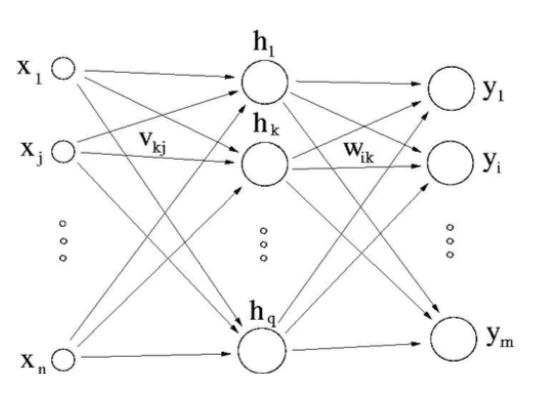
\includegraphics[width=8cm]{assets/mlp}
	\caption{Viacvrstvová dopredná neurónová sieť}
\end{figure}

Trénovací algoritmus pomocou ktorého sa trénujú dopredné neurónové sa nazýva "spätné šírenie chyby" (angl. backpropagation).

Aktivácie na neurónoch výstupnej vrstvy (výstup) môžeme popísať vzťahom:
\begin{equation}
y_i = f(\sum_{k=1}^{q+1}w_{ik}h_{k})
\end{equation}

Aktivácie na naurónoch skrytej vrstve môžeme popísať vzťahom:
\begin{equation}
	h_{k} = f(\sum_{j=1}^{n+1}v_{kj}x_{j})
\end{equation}

Prahové hodnoty:
\begin{equation}
	x_{n+1} = h_{q+1} = -1
\end{equation}

Aby dopredná neurónová sieť vedela pracovať aj s nelineárnymi problémami, musí byť aktivačná funkcia neurónov
nejaká nelineárna diferencovateľná funkcia. 

Najpoužívanejšie aktivačné funkcie sú:

\begin{itemize}
	\item Logistická sigmoida
	\item Hyperbolický tangens
	
	\begin{figure}[H]
		\centering
		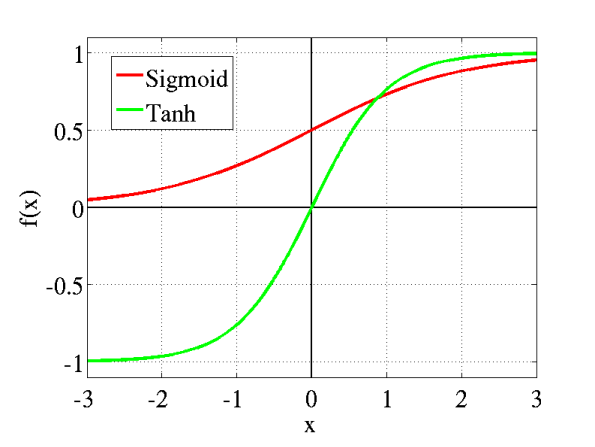
\includegraphics[width=8cm]{assets/activation_functions}
		\caption{Logistická sigmoida a Hyperbolický tangens}
	\end{figure}
	\item Relu
	\begin{figure}[H]
		\centering
		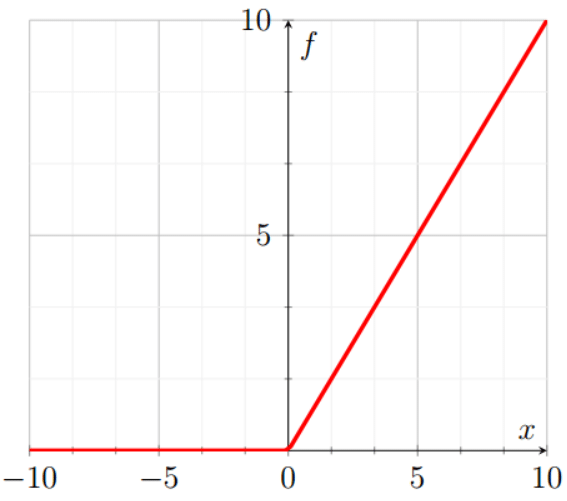
\includegraphics[width=8cm]{assets/relu}
		\caption{Rectified Linear Unit}
	\end{figure}
\end{itemize}

Vzťahy pre aktualizáciu váh sú nasledovné: \\

Váhy medzi vstupnou a skrytou vrstvou
\begin{equation}
	w_{ik}(t+1) = w_{ik}(t) + \alpha\delta_{i}h_{k} \quad \delta_{i} = (d_i - y_i)f'(net_{i})
\end{equation}

Váhy medzi skrytou a výstupnou vrstvou: 
\begin{equation}
	v_{kj}(t+1) = v_{kj}(t) + \alpha\delta_{k}x_{j} \quad \delta_{k} = (\sum_{i} w_{ik}\delta_{i})f'(net_{k})
\end{equation}

\subsection{Trénovací algoritmus dopredných neurónových sietí}
\begin{enumerate}
	\item zoberie sa vstup $x^{(p)}$ a vypočíta sa výstup $y^{(p)}$ (dopredný krok)
	\item vypočíta sa chyba pomocou zvolenej chybovej funkcie
	\item vypočítame hodnoty $\delta_{i}$ a $\delta_{k}$  (spätný krok)
	\item upravíme váhy $\Delta w_{ik}$ a $\Delta w_{kj}$
	\item ak už boli použité všetky trénovacie príklady z trénovacej množiny pokračuj bodom 6. inak pokračuj bodom 1.
	\item ak bolo dosiahnuté nejaké zastavovacie kritérium, potom skonči, inak prepermutuj vstupy a pokračuj bodom 1.
\end{enumerate}
                         

\subsection{Rekurentné neurónové siete}
Rekurentná neurónová sieť je akákoľvek neurónová sieť, ktorá obsahuje množinu neurónov
v ktorých sa uchováva informácia o aktiváciach neurónov z predošlých krokov. Takéto neuróny
nazývame aj rekurentné neuróny a tvoria vrstvu, ktorá sa nazýva kontextová vrstva.
Týmto spôsobom je sieť rozšírená o vnútornú pamäť.

V mojej práci budem skúmať vlastnosti a pamäťovú hĺbku rekurentnej siete s elmanovou architektúrou, 
ktorá je znázornená na nasledujúcom diagrame.

\begin{figure}[H]
	\centering
	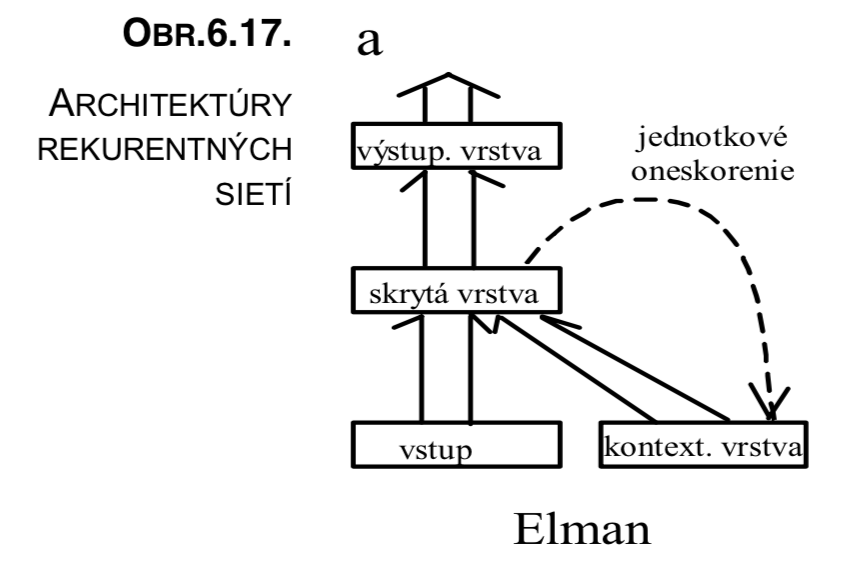
\includegraphics[width=8cm]{assets/elman_architecture}
	\caption{Architektúra elmanovej siete}
\end{figure}

Dvojité šípky reprezentujú spojenia neurónov medzi vrstvami. Neuróny v tej istej vrstve nie sú, podobne ako
v nerekurentnej doprednej sieti, medzi sebou prepojené. Spojenia znázornené dvojitou šípkou majú váhy, ktoré 
sú upravované počas trénovania.
Jednoduché šípky reprezentujú rekurentné spojenia. Tieto majú nemennú váhu s hodnotou 1.
Tieto spojenia slúžia na odpamätanie aktivácii rekurentných neurónov. 

Využitie rekurentných neurónových sietí:\\
\begin{itemize}
	\item Klasifikácia s časovým kontextom \\
	Príkladom úlohy môže byť napríklad určiť, či určitá postupnosť vstupov patrí do nejakej triedy.
	Praktickým problémom môže byť zistiť či postupnosť signálov z určitého zariadenia signalizuje poruchu zariadenia alebo nie
	\item Predikcie\\
	Príkladom môže byť napríklad predikcia nasledujúceho člena postupnosti
	\item Generovanie postupnosti\\
	Podobne ako predikcie, ale nepredikujeme iba ďalšiu hodnotu postupnosti, ale celé pokračovanie.
	Je to komplexnejšia úloha. Napríklad 23123123123123123123 .. pokračovaním by bolo 123123123...
	Reálne úlohy sú komplexnejšie.
\end{itemize}

Trénovací algoritmus, ktorým sa trénujú rekurentné neurónové siete
je spätné šírenie chyby v čase (ang. backpropagation through time)
Pri použití tohto algoritmu sa sieť rozvíja v čase, t.j. rozvinutá sieť má
toľko skrytých vrstiev, koľko je vstupov $T$ v stupnej postupnosti. 
Takáto sieť sa potom trénuje podobne ako klasická nerekurentná dopredná sieť s T skrytými vrstvami pomocou backpropagácie.
Aktivity neurónov kontextovej vrstvy sú na začiatku kažého cyklu trénovania nastavené
na hodnotu 0.5.


\begin{figure}[H]
	\centering
	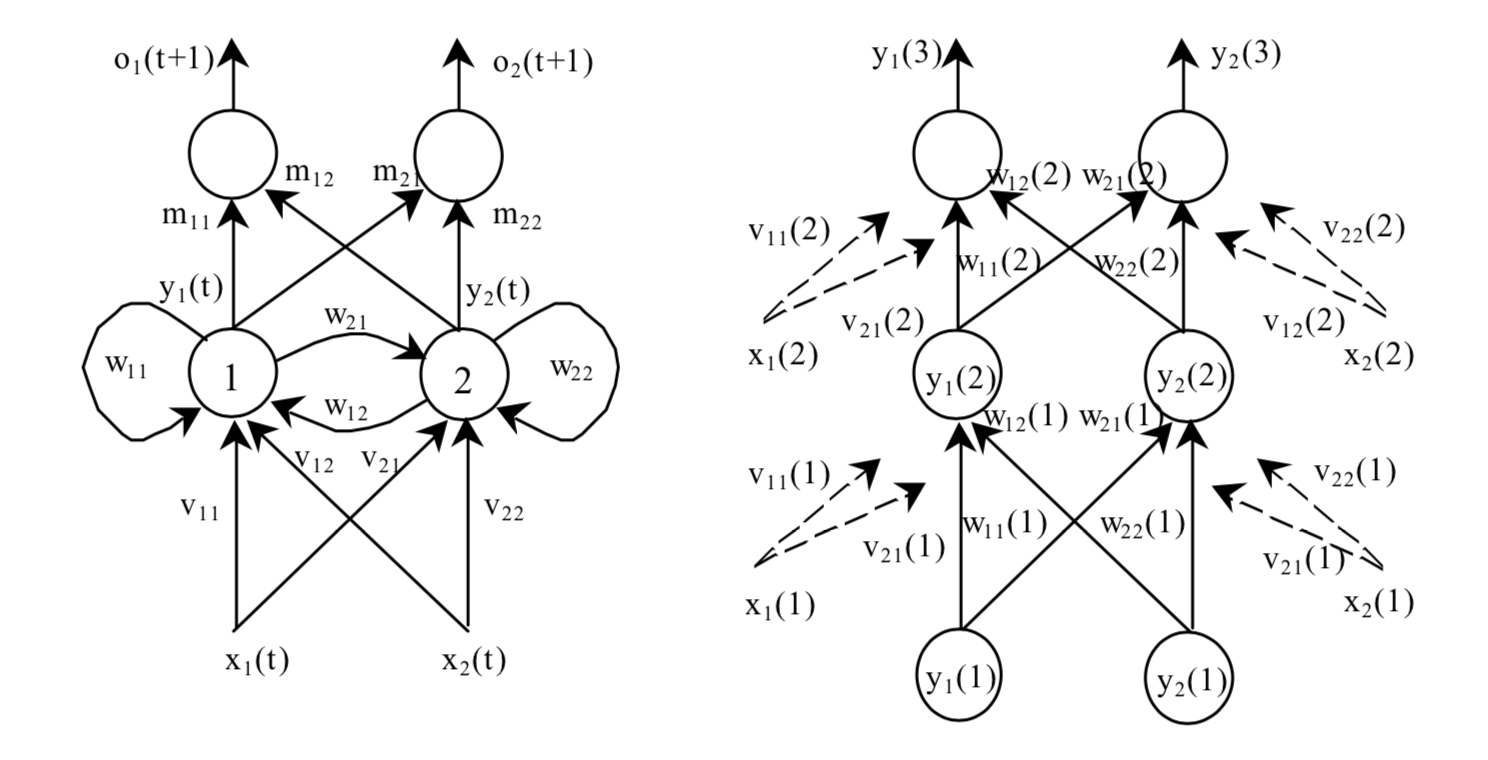
\includegraphics[width=8cm]{assets/elman}
	\caption{Rozvinutá elmanova sieť}
\end{figure}


Výstup takejto siete počítame pomocou vzťahu:

\begin{equation}
	o_{k}^(T+1) = f(\sum_{j-1}^{J}m_{kj}^{T+1}y_{j}^{T+1})
\end{equation}

\begin{equation}
	y_{j}^{t+1} = f (\sum_{i=1}^{J}w_{ji}^{t}y_{i}^{t} + \sum_{i=1}^{I}v_{ji}^{t}x_{i}^{t})
\end{equation}

Chybová funkcia  v čase $T + 1$
\begin{equation}
	E(T+1) = \frac{1}{2} \sum_{k+1}^{K}(d_{k}^(T+1) - o_{k}^(T+1))^{2}
\end{equation}

Zmena váh medzi vstupnou a výstupnou vrstvou:

\begin{equation}
	\Delta m_{kj}^{T+1} = -\alpha\frac{\partial E(T+1)}{\partial m_{kj}} = \alpha \delta_{k}^{T+1}y_{j}{T+1}
\end{equation}

\begin{equation}
	\delta_{k}^{T+1} = (d_{k}^{T+1} - o_{k}^{T+1})f'(net_{k}^{T+1})
\end{equation}

Váhy medzi rozvinutými vrstvami a medzi vzstupom a rozvinutými vrstvami sa upravujú pomocou vzťahov:

\begin{equation}
	\Delta w_{hj}^{T+1} = \frac{\sum_{t=1}^{T} \Delta w_{hj}^{t}}{T}
\end{equation}

\begin{equation}
	\Delta w_{ji}^{T+1} = \frac{\sum_{t=1}^{T} \Delta w_{ji}^{t}}{T}
\end{equation}



\subsection{Samoorganizujúce sa mapy}
Ďalším typom rekurentných neurónových sietí, ktorých pamäťovú hĺbku budeme 
skúmať v našej práci sú rekurentné samoorganizujúce sa mapy, 
ktoré sú rozšírením základnej nerekurentnej verzie samoorganizujúcich sa máp (ďalej iba SOM). 
Preto najskôr popíšem základný nerekurentný model SOM.

SOM je typ neurónovej siete, v ktorej sú jednotlivé neuróny usporiadané do (väčšinou) dvojrozmernej štvorcovej mriežky. Samoorganizujúce sa mapy (ďalej iba SOM) sú trénované bez učiteľa, čiže váhy jednotlivých neurónov sú upravované iba na základe dát z trénovacej množiny. 
Čo je zaujímavé na spôsobe trénovania SOM je, že je veľmi podobný učeniu neurónov v mozgovej kôre živočíchov. Je to biologicky inšpirovaný model.
Špeciálnou vlastnosťou SOM je, že po natrénovaní zobrazí trénovaciu množinu so zachovanou topológiou. To znamená, že blízke (podobné) vstupy aktivujú blízke neuróny v sieti. Vzdialenosť dvoch neurónov je ich euklidovská vzdialenosť v mriežke. Takéto topologické zobrazenie dát sa vyskytuje aj v biologických neurónových sieťach.

\subsection{Trénovanie}
Proces trénovania SOM je zložený z dvoch častí:
\begin{itemize}
\item hľadanie víťaza
\item adaptácia váh neurónov
\end{itemize}
Na začiatku su váhy medzi vstupom a neurónmi v mriežke inicializujú na náhodné hodnoty z určitého intervalu.
V každom kroku trénovania nájdeme najskôr víťazný neurón pre daný vstup. Postupne počítam euklidovské vzdialenosti vstupu od váhového vektora jednotlivých neurónov. Víťazom je neurón, ktorý je najbližšie k vstupu (má najkratšiu vzdialenosť).

\begin{equation}
i^* = argmin_i||x-w_i|| 
\end{equation}

Druhým krokom je adaptácia váh víťazného neurónu a jeho okolia. Pravidlo pre zmenu váh neurónov:

\begin{equation}
w_i(t+1) = w_i(t) + \alpha(t)h(i^*, i)([x(t) - w_i(t)])
\end{equation}

Váhové vektory víťazného neurónu a jeho topologických susedov sa posúvajú smerom k aktuálnemu vstupu.
$\alpha(t)$ predstavuje rýchlosť učenia, ktorá sa môže klesať v čase alebo môže zostať konštantná. Na funkcii, ktorá je použitá pre $\alpha$ v praxi veľmi nezaléží, mala by to byť nejaká monotónne klesajúca funkcia (napríklad exponenciálna funkcia). 
$h(i^*, i)$ je funkcia okolia (tzv. excitačná funkcia), ktorá definuje koľko neurónov v okolí víťaza bude trénovaných a do akej miery. Inými slovami, excitačná funkcia definuje rozsah kooperácie medzi neurónmi. Používajú sa najčastejšie 2 typy okolia:
\begin{itemize}
\item pravouhlé(štvorcové) okolie

\[
N(i^{*},i) =
     \begin{cases}
       \text{1} &\quad\text{ak } d_{M}(i^*, i) \leq \lambda(t) \\
       \text{0} &\quad\text{inak}\\
     \end{cases}
\]
\\
$d_{M}(i^{*}, i)$ je Manhattanovská vzdialenosť (L1 norma) medzi neurónmi v mriežke mapy. Kohonen zistil, že najlepšie výsledky sú dosiahnuté, keď
sa veľkosť okolia s časom postupne zmenšuje.
\item gaussovské okolie
	\begin{equation}
		N(i^{*}, i) = \exp^{- \frac{d^{2}_{E}(i^{*}, i)}{\lambda^{2}(t)}}
	\end{equation}
$d_{E}(i^{*}, i)$ je euklidovská vzdialenosť (L2 norma) neurónov v mriežke. Funkcia $\lambda^2(t)$ sa s časom postupne zmenšuje až k nule. Táto
	funkcia slúži na zmenšovanie okolia víťazného neurónu počas trénovania, čím sa zabezpečí ukončenie učenia.
\end{itemize}

$[x(t) - w_i(t)]$ Je euklidovská vzdialenosť medzi vstupným vektorom a váhovým vektorom.

Na vyhodnocovanie trénovania SOM používame kvantizačnú chybu. Je to vzdialenosť vstupu
od neurónu. 
Po každej epoche učenia vieme určiť celkovú kvantizačnú chybu siete pre danú trénovaciu množinu.
Vypočítame pre každý vstup vzdialenosť od každého neurónu v sieti. Spravíme priemer týchto vzdialeností pre každý vstup. Urobím súčet týchto hodnôt a vydelím počtom trénocích príkladov. 
Tým dostanem priemernu kvantizačnú chybu pre celú sieť. 
Táto by mala po každej epoche učenia (po natrénovaní a adaptácii váh na celej trénovacej množine) postupne klesať.

Pri učení rozlišujeme všeobecne dve fázy:
\begin{itemize}
	\item usporiadavanie - s časom klesá veľkosť okolia víťazných neurónov 
	\item dolaďovanie - veľkosť okolia sa zafixuje na nejakej malej hodnote až pokým učenie neskončí.
\end{itemize}

Kohonen odhadol na základe pokusov, že počet iterácií trénovania, by mal byť rádovo 500-násobok počtu neurónov v sieti.
Rovnako sa pozorovaním zistilo, že na fázu doladenia je lepšie ponechať viac času ako na fázu usporiadavania.

Počas trénovania SOM môžu nastať špeciálne situácie:

\begin{itemize}
	\item Sieť je neúplne rozvinutá - príliš rýchle zmenšovanie rýchlosti učenia $\alpha$
	\begin{figure}[H]
		\centering
		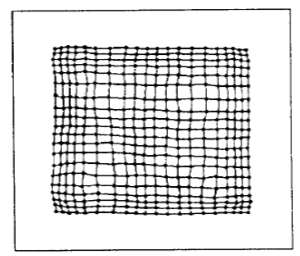
\includegraphics[width=8cm]{assets/too_fast}
		\caption{Neúplne rozvinutá sieť}
	\end{figure}
	
	\item Motýlí efekt - príliš rýchle zmenšovanie okolia $\lambda$
	\begin{figure}[H]
		\centering
		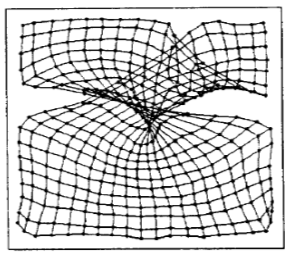
\includegraphics[width=8cm]{assets/butterfly_effect}
		\caption{Motýlí efekt}
	\end{figure}
	
	\item Pinch efekt - príliš pomalé zmenšovanie okolia $\lambda$
	\begin{figure}[H]
		\centering
		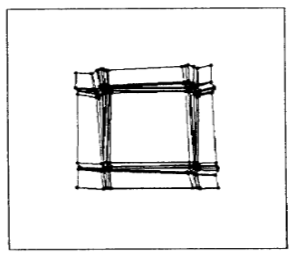
\includegraphics[width=8cm]{assets/pinch_effect}
		\caption{Pinch effect}
	\end{figure}
\end{itemize}

\subsection{Využitie SOM}
\begin{itemize}
\item SOM môžeme využiť na mapovanie viacrozmerných dát do 2D - môžeme ju použiť na redukciu dimenzie dát.
\item SOM je aj vektorovým kvantifikátorom. Pri vektorovej kvantizácii nahrádzame množinu vektorov vstupných dát menšou množinou vektorov (nazývaných aj prototypy). V SOM sú prototypmi
		váhové vektory. Toto je možné využiť napríklad na kompresiu dát. Vďaka vektorovej kvantizácii stačí uchovať iba množinu prototypov a informáciu o tom, ktorý vstupný vektor patrí 
		ku ktorému prototypu(centru). Ku každému centru sa potom priradí množina vstupných vektorov, ktoré ku nemu majú bližšie ako ku akémukoľvek inému centru. (používa sa euklidovská vzdialenosť).
		Vektorou kvantizáciou teda rozdelíme vstupný priestor an disjunktné oblasti, ktoré tvoria tzv. Voronoiho mozaiku
\end{itemize}


\subsection{Rekurentné modely}
Rekurentné samoorganizujúce sa mapy sú modifikáciou nerekurentnej SOM.
Rozdielom oproti nerekurentnej verzii je v tom, že vstupy sú porovnávané
nielen s váhovým vektorom jednotlivých neurónov, ale aj s kontextom.
Rôzne verzie rekurentných SOM sa líšia iba v type kontextu, ktorý je v nich použítý. 
V kontexte je spravidla uložený stav siete alebo časti siete z minulého časového kroku.

V mojej práci budem porovnávať 2 základné typy rekuretných SOM.

\begin{itemize}
	\item Recursive SOM (RecSOM)
	Pri RecSOM je kontextom celá kópia aktívacií neurónov z minulého kroku.
	\item Merge SOM (mSOM)
	Pri mSOM sú kontextom vlastnosti víťazného neurónu z predchádzajúceho kroku učenia.
\end{itemize}

\subsection{RecSOM}
Pri RecSom je SOM algoritmus použítý rekurzívne na vstupný vektor $x(t)$ a tiež reprezentáciu mapy
z minulého kroku $y(t-1)$. 

\begin{figure}[H]
	\centering
	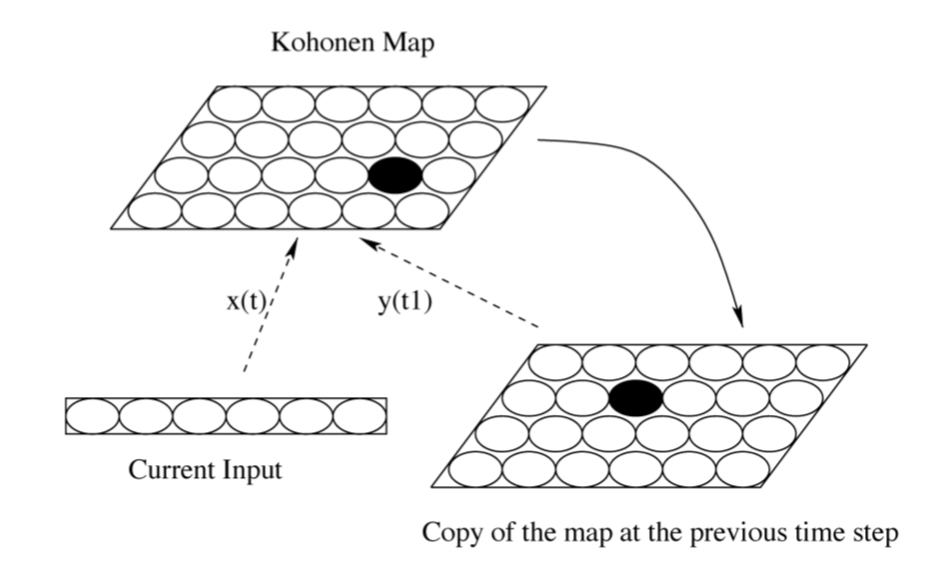
\includegraphics[width=10cm]{assets/rec_som}
	\caption{Architektúra RecSOM}
\end{figure}

V RecSOM je každý vstup asociovaný k stavom z predchádzajúcich krokov a preto každý 
neurón reaguje na sekvenciu vstupov.
Prerušované čiary predstavujú trénovateľné spojenia.

Každý neurón má 2 váhové vektory. Váhový vektor $w_i$, ktorý je porovnávaný so
vstupným vektorom $x(t)$ a vektor kontextových váh $c_i$, ktorý je porovnávaný s kontextom z predchádzajúceho
kroku $y(t-1)$. Kedže chceme aby boli dopredné a spätné spojenia v RecSOM homogénne, 
celkovú chybu určíme ako súčet druhých mocnín kvantizačných chýb oboch prípadov. Chyba je vlastne súčet euklidovských vzdialeností
vstupu od váhového vektoru a kontextu z predchádzajúceho kroku od kontextových váh. 

$N$ je počet neurónov v sieti (pretože kontextom je kópia celej mapy)
\begin{equation}
	d_i = \alpha \cdot ||x(t) - w_i||^{2} + b \cdot ||y(t-1) - c_i||^{2} \quad c \in R^{N}
\end{equation}
$\alpha$ a $\beta$ sú parametre, ktoré určujú akú váhu pri trénovaní bude mať kontext a akú váhu bude mať
aktuálny krok.

Kontextom je kópia aktivácii všetkých neurónov z predchádzajúceho kroku.
\begin{equation}
	y(t) = [y_1(t-1), ..., y_{N}(t-1)]  \quad c, r \in R^{N}
\end{equation}

Hodnota aktivácie pre určitý neurón je vyjadrená vzťahom:
\begin{equation}
	y_i = \exp(-d_i)
\end{equation}

Pravidlo pre zmenu váh neurónov (podobné ako pri nerekurentnej SOM):
\begin{equation}
	w_i(t + 1) = w_i(t) + \alpha(t)h(i^*, i)[x(t) - w_i(t)]
\end{equation}
Pre pre zmenu kontextových váh, platí to isté pravidlo ako pre normálne váhy, iba je aplikované 
na kontextové vektory:
\begin{equation}
	c_i(t + 1) = c_i(t) + \alpha(t)h(i^*, i)[y(t - 1) - c_i(t)]
\end{equation}

Pri RecSom majú kontext aj kontextové váhy veľkú dimenziu (rovnú počtu neurónov v sieti) čo môže spomalovať
proces trénovania.
Výhodou môže byť, že kontext RecSOM obsahuje veľa informácií a teda môže mať v niektorých prípadoch
lepšie vlastnosti. 


\subsection{mSOM}
mSOM je podobná recSOM, líši sa v reprezentácii kontextu.

Chybu (vzdialenosť vstupu od neurónu) vyjadríme vzťahom (podobne ako pri recSOM):
$d$ je dimenzia vstupov
\begin{equation}
	d_i = \alpha \cdot ||s(t) - w_i||^{2} + \beta \cdot ||r(t) - c_i||^{2} \quad x, c \in R^{d}
\end{equation}

Kontextom pri mSOM nie je kópia aktivácii neurónov z predchádzajúceho kroku, ako je tomu pri RecSom. 
Kontextom pri mSOM je zlúčenie (lineárna kombinácia) vlastností víťaza z predchádzajúceho kroku.
(Odtiaľ je odvodený názov - "zlučovacia samoorganizujúca sa mapa" - Merge SOM). 
Kontext mSOM vyjadríme vzťahom:
\begin{equation}
	y(t) = \beta \cdot w_{i^{*}}(t-1) + (1 - \beta) \cdot y_{i^{*}}(t-1)
\end{equation}
$\beta$ je zlučovací parameter, ktorý určuje váhu kombinovaných vlastností
víťazného neurónu z predchádzajúceho kroku. Typická hodnota tohto parametra
počas trénovania je $\beta = 0.5$, čiže taká aby obe zložky mali približne 
rovnakú váhu. Kontextom pri mSOM je teda lineárna kombinácia váhového vektora a 
kontextového vektora víťazného neurónu z predchádzajúceho kroku.
Pravidlá pre zmenu váh a kontextových váh zostávajú rovnaké ako pri RecSom, resp. SOM. Líšia sa iba v kontexte.
\begin{equation}
	w_i(t + 1) = w_i(t) + \alpha(t)h(i^*, i)[s(t) - w_i(t)]
\end{equation}
Pravidlo pre zmenu kontextových váh:
\begin{equation}
	c_i(t + 1) = c_i(t) + \alpha(t)h(i^*, i)[y(t - 1) - c_i(t)]
\end{equation}

Kontext pri mSOM obsahuje odlišné informácie ako pri RecSom.
Na rozdiel od recSom, kde kontext tvorí vektor aktivít neurónov z predchádzajúceho kroku, pri
mSOM je kontext tvorený iba lineárnou kombináciou vlastností víťazného neurónu z minulého kroku.
Má však menšiu dimenziu (dimenziu vstupu), vďaka čomu je trénovanie mSOM rýchlejšie a teda je možné použiť 
viacrozmerné mapy a viac epoch trénovania. Rozdielne typy kontextov a ich 
vplyv na pamäťovú hĺbku rekurentných sietí je jedným z cieľov mojej diplomovej práce.








